%% LyX 2.1.4 created this file.  For more info, see http://www.lyx.org/.
%% Do not edit unless you really know what you are doing.
\documentclass[english]{article}
\usepackage[T1]{fontenc}
\usepackage[latin9]{inputenc}
\usepackage{float}
\usepackage{url}
\usepackage{graphicx}

\makeatletter
\@ifundefined{showcaptionsetup}{}{%
 \PassOptionsToPackage{caption=false}{subfig}}
\usepackage{subfig}
\makeatother

\usepackage{babel}
\begin{document}

\title{Parametric Equations of the Oloid}


\author{logicmonkey}

\maketitle

\section*{Introduction}

The Oloid is a developable or torse or ruled surface. It is based
upon joining the points between two identical circles, perpendicular
to one another in space and separated such that each has its centre
lying on the circumference of the other. Points on one circle are
then joined to points on the other with a straight line - hence a
``ruled surface''.

The parametrization of the unit circle in the plane and centred at
the origin is typically given as ($\sin\left(t\right)$, $\cos\left(t\right)$)
over $t$\ensuremath{\in}$[-\pi,\pi)$. This is a good basis for the
parametrization of one of the circles, but not for the other. As will
be demonstrated, for the remarkable properties of the Oloid to be
realised, the mapping of a point on one circle to its corresponding
straight line end point on the other circle requires the arc of the
end point to have a different parametrization to that of the start.
Implementations that assume a naive connection of points typically
exhibit concave surfaces and are not Oloids. I call such surfaces
Fauxloids.

A derivation is given for the equations provided in \cite{key-1}.
A further alternative parametrization with a rational goal is also
shown and when rendered with a low polygon count approximates the
ideal more accurately.


\section*{Inversion with Respect to a Circle}

Point $A$ on the unit circle centred at the origin $O$ lies on the
tangent line that crosses the x-axis at point $P$ as shown in figure
\ref{fig:1}. The point $P'$ is the \textit{inverse} of $P$ with
respect to the circle. Similarly, $P$ is the inverse of $P'$. If
the x coordinate of $P'$ is $\cos\left(t\right)$, then the x coordinate
of $P$ is $\frac{1}{cos(t)}$. This bidirectional relationship is
exploited in the following sections.

\noindent \begin{center}
\begin{figure}[H]
\noindent \begin{centering}
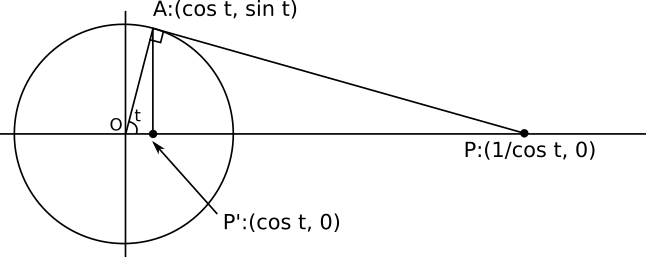
\includegraphics[scale=0.5]{lm_inversion}
\par\end{centering}

\centering{}\caption{Inversion with respect to a circle\label{fig:1}}
\end{figure}

\par\end{center}


\section*{Parametrization using Transcendental Functions}

Points $U$ and $V$ lie on unit circles centred at $C_{U}=(0,-\frac{1}{2})$
and $C_{V}=(0,\frac{1}{2})$ respectively as shown in figure \ref{fig:2}.
$U$ and $V$ correspond to points $A$ and $B$ in \cite{key-1}.

\begin{equation}
U\left(t\right)=\left[\sin\left(t\right),-\frac{1}{2}-\cos\left(t\right),0\right]\label{eq:1}
\end{equation}


The triangle $T'UV$ is formed by the joining line $UV$ and the intersection
point $T'$ of the tangent lines through $U$ and $V$. Point $T'$
is also the inverse of point $T_{U}=(0,-\frac{1}{2}-\cos\left(t\right))$. 

By inversion with respect to the circle, the distance $C_{U}T'$ is
\[
|C_{U}T'|=\frac{1}{\cos\left(t\right)}
\]


\noindent 
\begin{figure}[H]
\noindent \centering{}\subfloat[]{\noindent \begin{centering}
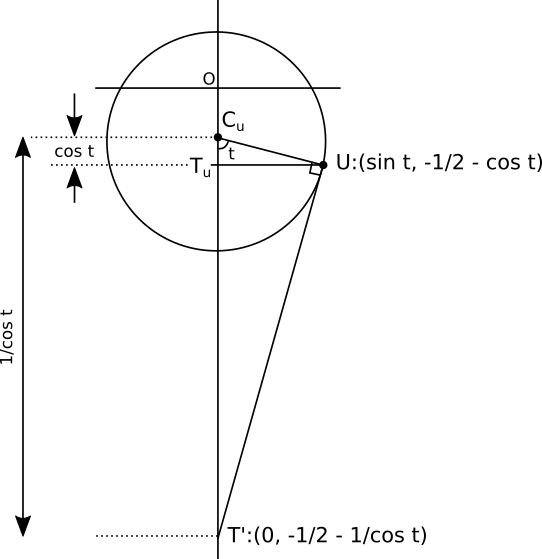
\includegraphics[scale=0.7]{ds1}
\par\end{centering}

}\subfloat[]{\noindent \begin{centering}
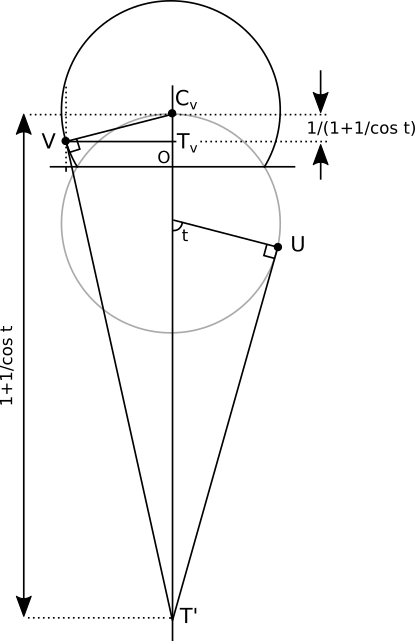
\includegraphics[scale=0.7]{ds2}
\par\end{centering}

}\caption{Distances $|C_{U}T'|$and $|T'C_{V}|$\label{fig:2}}
\end{figure}


For simplicity, the circle centred at $C_{V}$ is rotated from yz
into the xy plane. Since the circle centres are unit distance apart,
the length $T'C_{V}$ is therefore

\[
|T'C_{V}|=1+\frac{1}{\cos\left(t\right)}
\]
$T_{V}$ is the inverse of $T'$ with respect to the upper circle,
making the displacement along the y axis

\[
|C_{V}T_{V}|=\frac{1}{1+\frac{1}{\cos\left(t\right)}}=\frac{\cos\left(t\right)}{1+\cos\left(t\right)}
\]


\noindent By Pythagoras, the squared distance of $V$ to the y axis
is 
\[
|VT_{V}|^{2}=1-\frac{\cos^{2}\left(t\right)}{\left(1+\cos\left(t\right)\right)^{2}}=\frac{1+2\cos\left(t\right)}{\left(1+\cos\left(t\right)\right)^{2}}
\]


\noindent Rotating back into the yz plane it follows that V has the
parametrization

\begin{equation}
V\left(t\right)=\left[0,\frac{1}{2}-\frac{\cos\left(t\right)}{1+\cos\left(t\right)},\pm\frac{\sqrt{1+2\cos\left(t\right)}}{1+\cos\left(t\right)}\right]\label{eq:2}
\end{equation}



\section*{Alternative Quasi-Rational Parametrization}

The approach taken for an alternative parametrization is identical
to the one already given. This time as shown in figure \ref{fig:3},
the rational parametrization of the circle is used as a starting point

\begin{equation}
U\left(t\right)=\left[\frac{2t}{1+t^{2}},-\frac{1}{2}-\frac{1-t^{2}}{1+t^{2}},0\right]\label{eq:3}
\end{equation}


\noindent \begin{center}
\begin{figure}[H]
\begin{centering}
\subfloat[]{\noindent \centering{}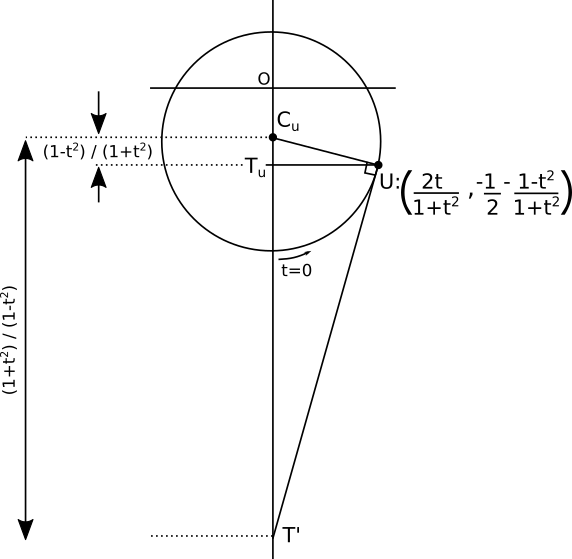
\includegraphics[scale=0.7]{lm1}}\subfloat[]{\noindent \centering{}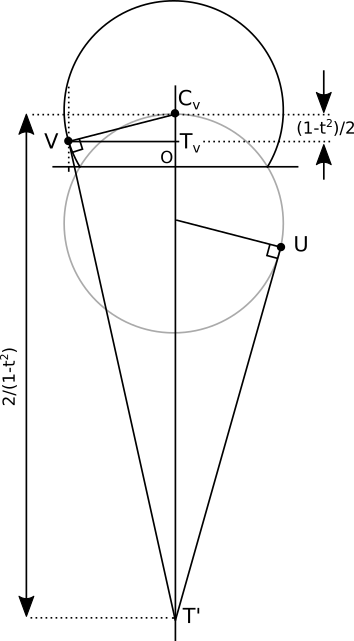
\includegraphics[scale=0.7]{lm2}}
\par\end{centering}

\centering{}\caption{Alternative rational parametrization\label{fig:3}}
\end{figure}

\par\end{center}

\noindent It follows that

\begin{equation}
V\left(t\right)=\left[0,\pm\frac{1}{2}\sqrt{\left(3-t^{2}\right)\left(1+t^{2}\right)},\frac{t^{2}}{2}\right]\label{eq:4}
\end{equation}



\section*{Comparison of the Parametrizations}

When rendered in a 3D graphics program, both parametrizations give
pleasing results. The first method uses $t\in\left[-\frac{2}{3}\pi,\frac{2}{3}\pi\right]$while
the second uses $t\in\left[-\sqrt{3},\sqrt{3}\right]$. There is no
escape from irrational constants in the second method despite its
rational intentions.

\noindent \begin{center}
\begin{figure}[H]
\noindent \subfloat[Original\label{fig:4a}]{\noindent \begin{centering}
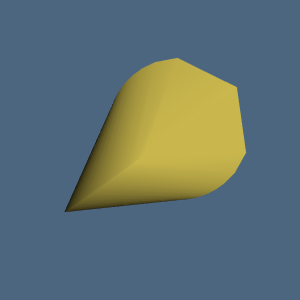
\includegraphics[scale=0.5]{Oloid28}
\par\end{centering}

\noindent \centering{}}\subfloat[Quasi-rational\label{fig:4b}]{\noindent \begin{centering}
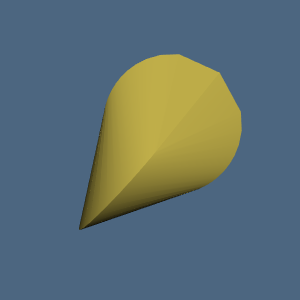
\includegraphics[scale=0.5]{rOloid28}
\par\end{centering}

\noindent \centering{}}\caption{Comparison of Oloids using 28 sub-divisions per circular arc\label{fig:4}}
\end{figure}

\par\end{center}

Figures \ref{fig:4a} and \ref{fig:4b} show the Oloid rendered with
a low polygon count. The quasi-rational parametrization is appreciably
closer to the ideal. Figure \ref{fig:5} shows how both parametrizations
project the circular arc traced by $V$ on the plane and their different
trajectories. The vertical axis tracks the parameter $t$. The steeper
slope of the original parametrization indicates a less uniform distribution
of sample points than the quasi-rational solution. This is reflected
in the relative surface quality at low polygon counts.

\noindent \begin{center}
\begin{figure}[H]
\noindent \begin{centering}
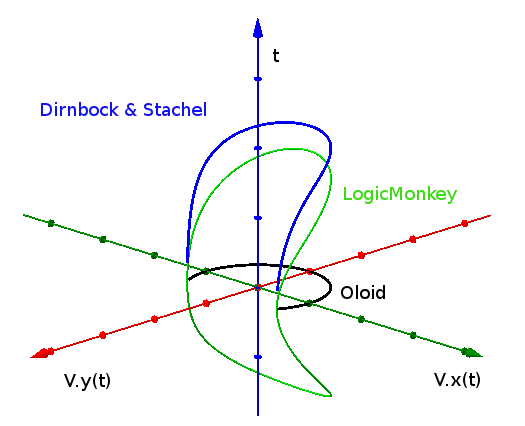
\includegraphics{Oloid-arc-param}
\par\end{centering}

\centering{}\caption{Functions over full range of parameter $t$\label{fig:5}}
\end{figure}

\par\end{center}

The property $|UV|=\sqrt{3}$ is readily proven using equations \ref{eq:1}
and \ref{eq:2} as in \cite{key-1}. Demonstrating the same with equations
\ref{eq:3} and \ref{eq:4} has so far eluded the author.


\section*{C++ Source Code using VTK}

\noindent \begin{flushleft}
\url{https://github.com/logicmonkey/surfaces/blob/master/Oloid/Oloid.cxx}
\par\end{flushleft}

\noindent \begin{flushleft}
\url{https://github.com/logicmonkey/surfaces/blob/master/rOloid/rOloid.cxx}
\par\end{flushleft}
\begin{thebibliography}{1}
\bibitem[1]{key-1}Dirnbock H., Stachel H. The Development of the
Oloid. Journal for Geometry and Graphics Volume 1 (1997), No. 2, 105\textendash 118\end{thebibliography}

\end{document}
